\section{Prompts} \label{app:prompts}

In this section, we outline the various prompting methods used for the different evaluations we conducted, along with example solutions for each evaluation

\subsection{Chain-of-Thought Solver}
For our main results, presented in~\cref{tab:main_results}, we use a direct approach where each model is asked to solve the problem. We further give instructions for the precise way in which the answer should be formatted. 

% !TEX root = main.tex

\begin{figure}[t]
\vspace{-1.5cm}
\begin{minipage}{0.34\textwidth}
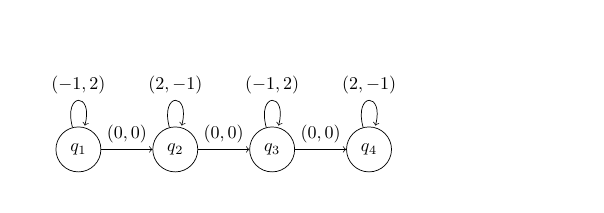
\begin{tikzpicture}[scale=0.25]
\usetikzlibrary{automata, positioning}
\scalebox{0.65}{
\node[state] (q1) {$q_1$};
\node[state, right=of q1] (q2) {$q_2$};
\node[state, right=of q2] (q3) {$q_3$};
\node[state, right=of q3] (q4) {$q_4$};

\path[->] (q1) edge [loop above] node[above] {$(-1,2)$} (q1) edge node[above] {$(0,0)$} (q2); 
\path[->] (q2) edge [loop above] node[above] {$(2,-1)$} (q2) edge node[above] {$(0,0)$} (q3);
\path[->] (q3) edge [loop above] node[above] {$(-1,2)$} (q3) edge node[above] {$(0,0)$} (q4);
\path[->] (q4) edge [loop above] node[above] {$(2,-1)$} (q4);
}
\end{tikzpicture}
\end{minipage}
\begin{minipage}{0.32\textwidth}
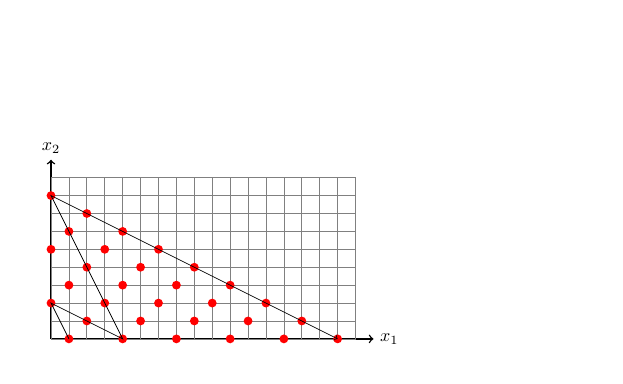
\begin{tikzpicture}[scale=0.35]
\scalebox{0.65}{
\draw[->, thick] (0, 0) -- (18, 0) node[right] {$x_1$};
\draw[->, thick] (0, 0) -- (0, 10) node[above] {$x_2$};

\draw[step=1, gray, thin] (0, 0) grid (17, 9);

\foreach \x in {1,4,7,10,13,16} \fill[red] (\x,0) circle (7pt);
\foreach \x in {2,5,8,11,14} \fill[red] (\x,1) circle (7pt);
\foreach \x in {0,3,6,9,12} \fill[red] (\x,2) circle (7pt);
\foreach \x in {1,4,7,10} \fill[red] (\x,3) circle (7pt);
\foreach \x in {2,5,8} \fill[red] (\x,4) circle (7pt);
\foreach \x in {0,3,6} \fill[red] (\x,5) circle (7pt);
\foreach \x in {1,4} \fill[red] (\x,6) circle (7pt);
\foreach \x in {2} \fill[red] (\x,7) circle (7pt);
\foreach \x in {0} \fill[red] (\x,8) circle (7pt);

\draw[->] (1,0) -- (0,2) -- (2,1) -- (4,0) -- (3,2) -- (2,4) -- (1,6) -- (0,8) -- (2,7) -- (4,6) -- (6,5) -- (8,4) -- (10,3) -- (12,2) -- (14,1) -- (16,0);
}
\end{tikzpicture}
\end{minipage}
\begin{minipage}{0.32\textwidth}
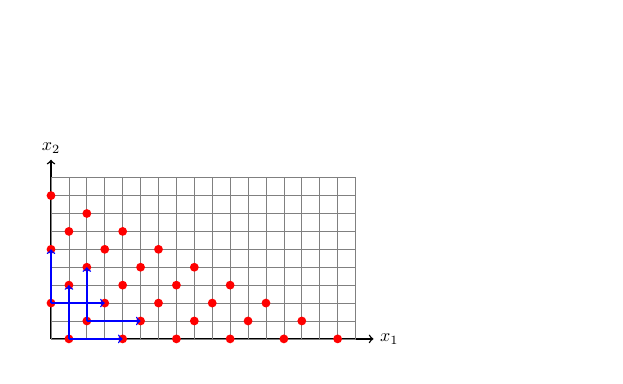
\begin{tikzpicture}[scale=0.35]
\scalebox{0.65}{
\draw[->, thick] (0, 0) -- (18, 0) node[right] {$x_1$};
\draw[->, thick] (0, 0) -- (0, 10) node[above] {$x_2$};

\draw[step=1, gray, thin] (0, 0) grid (17, 9);

\foreach \x in {1,4,7,10,13,16} \fill[red] (\x,0) circle (7pt);
\foreach \x in {2,5,8,11,14} \fill[red] (\x,1) circle (7pt);
\foreach \x in {0,3,6,9,12} \fill[red] (\x,2) circle (7pt);
\foreach \x in {1,4,7,10} \fill[red] (\x,3) circle (7pt);
\foreach \x in {2,5,8} \fill[red] (\x,4) circle (7pt);
\foreach \x in {0,3,6} \fill[red] (\x,5) circle (7pt);
\foreach \x in {1,4} \fill[red] (\x,6) circle (7pt);
\foreach \x in {2} \fill[red] (\x,7) circle (7pt);
\foreach \x in {0} \fill[red] (\x,8) circle (7pt);

\draw[->,blue,thick] (1,0) -- (4,0);
\draw[->,blue,thick] (1,0) -- (1,3);

\draw[->,blue,thick] (2,1) -- (5,1);
\draw[->,blue,thick] (2,1) -- (2,4);

\draw[->,blue,thick] (0,2) -- (3,2);
\draw[->,blue,thick] (0,2) -- (0,5);
}
\end{tikzpicture}
\end{minipage}
\caption{Left: 4-component \dvass $V_2$. 
Middle: the set $\reach_{q_4}(V_2, q_1(1,0))$ and a path $q_1(1,0) \tran q_4(16,0)$.
Right: bases 
%$A = \{(1,0),(2,1),(0,2)\}$ 
and periods 
%$P = \{(0,3),(3,0)\}$
 of an over-approximating semi-linear set $A+P^*$.}
\label{fig:zigzag}
\end{figure}

\begin{example}
For $k\geq 1$, let $V_k$ be a $(2k)$-component \dvass, where each component has just one state $q_i$
and one transition:
$(q_i, (-1,2), q_i)$ for odd $i$, and $(q_i, (2,-1), q_i)$ for even $i$.
Bridge transitions are $(q_i, (0,0), q_{i+1})$.
Figure~\ref{fig:zigzag} shows $V_2$ (left) and 
a path in $V_2$ from $s = q_1(1,0)$ to $t = q_4(16,0)$ together with 
the reachability set $\reach_{q_4}(V_2, s)$ (middle).
In general,
\begin{align} \label{eq:reachk}
X_k := \reach_{q_{2k}}(V_k, s) \ = \ \set{(x_1,x_2) \mid x_1+2x_2 \leq 4^k, \  x_1+2x_2 \equiv 1 \!\! \mod 3}.
\end{align}
Even if the size of the reachability set is 
exponential in $k$, for small $(x_1, x_2)$ it is periodic and the periods are small.
The set $X_k$ can be over-approximated by $A + P^*$ for $A = \set{(1,0),(2,1),(0,2)}$ and $P = \set{(0,3),(3,0)}$
(shown on the right of Figure~\ref{fig:zigzag}), namely for every $k\geq 1$ and $B\in\N$,
the set $X_k$ is \kanapka {$8$} {$B$}. 
For illustration, consider $Y := X_k \cap ((1,0) + P^*)$.
If $(1,0) + P^{\leq B} \subseteq X_k$ then $Y$ is a $B$-approximation
of $(1,0) + P^*$ with $\norm((1,0)), \norm(P) \leq 3 \leq 8$. 
Otherwise, there is some $(v_1, v_2) \in \big((1,0) + P^{\leq B}\big)\setminus X_k$, and
then $B$ is larger than $4^k$:
\[
%8B \geq 2(1 + 3B) \geq 2(v_1 + v_2) \geq v_1 + 2 v_2 > 
4^k < v_1 + 2 v_2 \leq 2(v_1 + v_2) \leq 2(1+3B) \leq 8B.
\]
Therefore by \eqref{eq:reachk}, each $(x_1,x_2) \in Y$ satisfies 
$\norm(x_1,x_2) = x_1 + x_2 \leq x_1 + 2x_2 \leq 4^k < 8B$, and thus
$Y$, seen as a union of singletons, is a union of 
linear sets with norm of base bounded by $8B$ and empty set of periods. 
In both cases, 
$Y$ is \kanapka {$8$} {$B$}. 
%The same intuition stays behind polynomial approximability of \dvass stated in Lemma~\ref{lem:2vass-sandwich}.
\end{example}

\newpage

\subsection{Coding Agent}
The coding agents are allowed to run any code they deem necessary. We give instructions on how this can be done, as below:


\begin{prompt}{Prompt}
Let $n \geq 2$ be an integer. Consider an $n \times n$ chessboard divided into $n^2$ unit squares.
We call a configuration of $n$ rooks on this board *happy* if every row and every column contains exactly one rook. 
For $n=22$ and $k=5$, find a happy configuration of rooks such that there is no $k \times k$ square without a rook on any of its $k^2$ unit squares.

Format your reply as follows:
Output a comma-separated list of 1-based rook indices (so (1, 1) is the top left corner of the board) inside of $\boxed{...}$, for example $\boxed{((1,1), (4,5), (1,6))}$.
\end{prompt}

\begingroup\raggedleft
\begin{geminils}{\geminiflheader}
Okay, I understand the problem. We need to find a happy configuration of 22 rooks on a 22x22 chessboard such that no 5x5 square is empty of rooks. A happy configuration means there's exactly one rook in each row and each column. This is equivalent to a permutation of the numbers from 1 to 22. The condition that no 5x5 square is empty is the crucial constraint. A simple permutation like (1, 1), (2, 2), ..., (22, 22) would not satisfy this condition. If we place the rooks on the main diagonal, then any 5x5 subgrid along the diagonal has no rooks in the upper-right 4x4 corner or the bottom-left 4x4 corner, so it does not work. To ensure no 5x5 square is empty, we need to spread the rooks out somewhat evenly. A good starting point might be to place the rooks on the main diagonal and then offset each rook by a certain amount. Consider placing rooks at (i, a * i mod n + 1) for a constant a. 
Let's try with a=1. The rooks are at (i, i). This doesn't work. 
Let's try a=2. (i, 2*i mod 22 + 1) 
Let's try a=3. (i, 3*i mod 22 + 1).
Let's try the configuration where the $i$-th rook is at position $(i, 3i \\pmod{22} + 1)$, where the indices are 1-based. This is guaranteed to have one rook per row. We need to check if there is one rook per column. If we map $i \\to 3i \\pmod{22}$, this map is a permutation since 3 and 22 are coprime. Hence this is a valid rook configuration.
Now we need to see if there's a 5x5 subgrid with no rooks. I will generate the configuration for $n=22$ using $a=3$ and then visually check whether it might work. 
```python
n = 22
a = 3
rooks = []
for i in range(1, n + 1):
    col = (a * i) \% n + 1
    rooks.append((i, col))
    
    print(rooks)

def check_5x5_empty(rooks, n):
    for r in range(1, n - 4 + 1):
        for c in range(1, n - 4 + 1):
            empty = True
            for row in range(r, r + 5):
                for col in range(c, c + 5):
                    if (row, col) in rooks:
                        empty = False
                        break
                if not empty:
                    break
            if empty:
                print(f"5x5 empty square found at ({r}, {c})")
                return False
    return True

print(check_5x5_empty(rooks, n))```
\end{geminils}
\endgroup

\begin{prompt}{User}
Code Output:
```[(1, 4), (2, 7), (3, 10), (4, 13), (5, 16), (6, 19), (7, 22), (8, 3), (9, 6), (10, 9), (11, 12), (12, 15), (13, 18), (14, 21), (15, 2), (16, 5), (17, 8), (18, 11), (19, 14), (20, 17), (21, 20), (22, 1)]
5x5 empty square found at (1, 17)
False
\end{prompt}

\begingroup\raggedleft
\begin{geminils}{\geminiflheader}
Okay, the code output shows that the configuration with $a=3$ doesn't work. It found a 5x5 empty square. Let's try $a=7$.
```python
n = 22
a = 7
rooks = []
for i in range(1, n + 1):
    col = (a * i) \% n + 1
    rooks.append((i, col))
    
    print(rooks)

def check_5x5_empty(rooks, n):
    for r in range(1, n - 4 + 1):
        for c in range(1, n - 4 + 1):
            empty = True
            for row in range(r, r + 5):
                for col in range(c, c + 5):
                    if (row, col) in rooks:
                        empty = False
                        break
                if not empty:
                    break
            if empty:
                print(f"5x5 empty square found at ({r}, {c})")
                return False
    return True

print(check_5x5_empty(rooks, n))```
\end{geminils}
\endgroup

\begin{prompt}{User}
Code Output:
```[(1, 8), (2, 15), (3, 22), (4, 7), (5, 14), (6, 21), (7, 6), (8, 13), (9, 20), (10, 5), (11, 12), (12, 19), (13, 4), (14, 11), (15, 18), (16, 3), (17, 10), (18, 17), (19, 2), (20, 9), (21, 16), (22, 1)]
5x5 empty square found at (1, 1)
False
\end{prompt}

\begingroup\raggedleft
\begin{geminils}{\geminiflheader}
Okay, $a=7$ also doesn't work. Let's try $a=9$.
```python
n = 22
a = 9
rooks = []
for i in range(1, n + 1):
    col = (a * i) \% n + 1
    rooks.append((i, col))
    
    print(rooks)

def check_5x5_empty(rooks, n):
    for r in range(1, n - 4 + 1):
        for c in range(1, n - 4 + 1):
            empty = True
            for row in range(r, r + 5):
                for col in range(c, c + 5):
                    if (row, col) in rooks:
                        empty = False
                        break
                if not empty:
                    break
            if empty:
                print(f"5x5 empty square found at ({r}, {c})")
                return False
    return True

print(check_5x5_empty(rooks, n))```
\end{geminils}
\endgroup

\begin{prompt}{User}
Code Output:
```[(1, 10), (2, 19), (3, 6), (4, 15), (5, 2), (6, 11), (7, 20), (8, 7), (9, 16), (10, 3), (11, 12), (12, 21), (13, 8), (14, 17), (15, 4), (16, 13), (17, 22), (18, 9), (19, 18), (20, 5), (21, 14), (22, 1)]
True
\end{prompt}
    
\begingroup\raggedleft
\begin{geminils}{\geminiflheader}
Okay, the code output shows that the configuration with $a=9$ works!
The rook positions are: (1, 10), (2, 19), (3, 6), (4, 15), (5, 2), (6, 11), (7, 20), (8, 7), (9, 16), (10, 3), (11, 12), (12, 21), (13, 8), (14, 17), (15, 4), (16, 13), (17, 22), (18, 9), (19, 18), (20, 5), (21, 14), (22, 1).
Final Answer: The happy configuration of rooks is \\boxed{((1, 10), (2, 19), (3, 6), (4, 15), (5, 2), (6, 11), (7, 20), (8, 7), (9, 16), (10, 3), (11, 12), (12, 21), (13, 8), (14, 17), (15, 4), (16, 13), (17, 22), (18, 9), (19, 18), (20, 5), (21, 14), (22, 1))}.
\end{geminils}
\endgroup


\begin{parsecheckcorrect}{Parsed Answer - Correct}
[[1, 10], [2, 19], [3, 6], [4, 15], [5, 2], [6, 11], [7, 20], [8, 7], [9, 16], [10, 3], [11, 12], [12, 21], [13, 8], [14, 17], [15, 4], [16, 13], [17, 22], [18, 9], [19, 18], [20, 5], [21, 14], [22, 1]]
\end{parsecheckcorrect}


\subsection{Bruteforce Solver}
For the brute-force approach, the models are asked to generate a single block of code that naively creates a solution satisfies the problem's constraints. Only one attempt to produce the code is permitted.
\begin{system}{System}
You are an expert mathematician that solves problems using a brute-force approach. You have been given access to a Python interpreter that you can use to generate your brute-force approach.
Make sure to abide by the following rules:
    1. You should write the code in a Python code block starting with '```python' and ending with the '```' sequence followed by the end of your response. 
    2. The code should be a brute-force solution without optimizations. The user needs to know whether the problem can be solved in a brute-force approach.
    3. After you have written your code, you can immediately stop your output. The user will execute your code and give you the results. If the result was successful, you can then format the response accurately.
    4. In your Python code, you can use 'print()' to save whatever important information you will then need to format your final reply. The user will then execute your code in a Python environment.
    5. Your code will run for two minutes. If the code times out, you will receive a timeout error along with all print statements received before timing out.
    6. Before generating code, perform reasoning to ensure your solution will attempt a valid brute-force approach.
    7. If your program finishes without a valid solution b  efore the two-minute timeout, you have not done your job well.
\end{system}

\begin{prompt}{User}
Given $n = 27$, find a sequence of distinct real numbers $x_1, \ldots, x_n$ such that each of the sets$\{x_1, x_2, x_3\}, \{x_2, x_3, x_4\},\ldots,\{x_{n-2}, x_{n-1}, x_n\}, \{x_{n-1}, x_n, x_1\},\text{ and } \{x_n, x_1, x_2\}$ forms a 3-term arithmetic progression when arranged in increasing order.
\end{prompt}

\begingroup\raggedleft
\begin{claudels}{\claudeheader}
Let me reason about this problem:  
    1) We need to find 27 distinct numbers where each consecutive triplet forms an arithmetic sequence when sorted 
    2) The triplets wrap around, meaning the last two numbers connect with the first ones 
    3) A brute-force approach would be to:    
        - Start with some small initial values    
        - Incrementally try values that satisfy each consecutive triplet    
        - Keep track of used values to ensure distinctness    
        - Check if it wraps around correctly  
    4) For a brute-force solution, let's:    
        - Start with small initial values (x\u2081, x\u2082)    
        - For each next value, ensure it can form an AP with previous two when sorted    
        - Use reasonable bounds to limit search space    
        - Check for distinctness  
Let me write code to search for such a sequence:  

```python 
def is_arithmetic_when_sorted(a, b, c):     
    nums = sorted([a, b, c])     
    return abs((nums[1] - nums[0]) - (nums[2] - nums[1])) < 1e-10  

def check_sequence(seq):     
    n = len(seq)
    for i in range(n):
        if not is_arithmetic_when_sorted(seq[i], seq[(i+1)\%n], seq[(i+2)\%n]):             
            return False     
    # Check distinctness     
    return len(set(seq)) == len(seq)  

def find_sequence(n=27):     
    def extend_sequence(current_seq):         
        if len(current_seq) == n:             
            if check_sequence(current_seq):                 
                print(','.join(map(str, current_seq)))                 
                return True             
            return False 

        prev1, prev2 = current_seq[-2:]

        # Try values that could potentially form arithmetic sequence         
        used = set(current_seq)

        # Try different possibilities for next value         
        for multiplier in range(-10, 11):             
            # Try extending based on arithmetic patterns            
            candidates = [                 
                2 * prev2 - prev1 + multiplier,  # Continue AP in one direction                 
                2 * prev1 - prev2 + multiplier,  # Continue AP in other direction                 
                (prev1 + prev2)/2 + multiplier   # Middle value             
            ]                          
            for next_val in candidates:                 
                if next_val not in used and -100 <= next_val <= 100:                     
                    if is_arithmetic_when_sorted(prev1, prev2, next_val):                         
                        if extend_sequence(current_seq + [next_val]):                             
                            return True         
        return False   
       
# Try different starting values     
for start in range(-5, 6):         
    for second in range(-5, 6):             
        if start != second:                 
            if extend_sequence([start, second]):                     
                return  find_sequence() ```
\end{claudels}
\endgroup

\begin{prompt}{User}
Code Output: 
```-5,-4,-6,-8,-10,-12,-14,-16,-18,-20,-22,-24,-26,-28,-30,-32,-34,-33,-35,-31,-27,-23,-19,-15,
-11,-7,-3```
This was the last time your code can be executed. From now on, you will not be able to execute code.
\end{prompt}

\begingroup\raggedleft
\begin{claudels}{\claudeheader}
Based on the output, I can now provide the solution.
$\boxed{-5,-4,-6,-8,-10,-12,-14,-16,-18,-20,-22,-24,-26,-28,-30,-32,-34,-33,-35,-31,-27,-23,-19,-15,}$
$\boxed{-11,-7,-3}$
This sequence satisfies all the required conditions:
    1. It contains 27 distinct numbers
    2. Each consecutive triplet forms an arithmetic sequence when arranged in increasing order
    3. The wrap-around condition is also satisfied (the last two numbers with the first, and the last number with the first two)
\end{claudels}
\endgroup

\begin{parsecheckcorrect}{Parsed Answer - Correct}
[-5, -4, -6, -8, -10, -12, -14, -16, -18, -20, -22, -24, -26, -28, -30, -32, -34, -33, -35, -31, -27, -23, -19, -15, -11, -7, -3]
\end{parsecheckcorrect}



\subsection{Brute+Infer Solver}
Unlike the pure brute-force solver, the brute-force inference agent is allowed to explore solutions with smaller parameters as to generalize the pattern. It is allowed up to two feedback rounds to explore settings and test different strategies. The interaction below demonstrates how a model, in this case GPT-4o, can adapt its naive brute-force approach into a more effective algorithm by combining logical reasoning with a programmatic solution.
\begin{system}{System}
You are an expert mathematician that solves problems using a brute-force approach and logical inference. You approach mathematical problems by first solving them in a brute-force manner for 
smaller cases if necessary and then generalizing your findings to solve the problem itself. In order to solve the problem, you need to progress in a series of steps. In each step, you can execute a Python code block to test your current idea.

Make sure to abide by the following rules:

    1. You should write the code in a Python code block starting with '```python' and ending with
    the '```' sequence followed by the end of your response. 
    2. Try to solve the problem in a brute-force manner for smaller cases (or for the case itself if possible) and then generalize your findings to solve the problem itself. Try to find patterns, relationships, or properties that can help you solve the problem.
    3. After you have written your code, you can stop your output. The user will execute your code and give you the results. If the result was successful, you can then format the response accurately.
    4. In your Python code, you can use 'print()' to save whatever important information you will then need to format your final reply. The user will then execute your code in a Python environment.
\end{system}

\begin{prompt}{User}
A divisor $d$ of a positive integer $n$ is said to be a close divisor of $n$ if $\sqrt{{60}} < d < 2\sqrt{{60}}$\Find a positive integer with exactly 60 close divisors.

Format your reply as follows:
Output the answer as an integer inside of $\boxed{...}$. For example $\boxed{123}$.\Your answer can contain mathematical operations using valid LaTeX notation.
\end{prompt}

\begingroup\raggedleft
\begin{gpt}{\gptheader}
    To solve this problem, we need to find a positive integer $n$ such that the number of its divisors $ d $ satisfying $ \sqrt{n} < d < 2\sqrt{n} $ is exactly 60. \\Let's break down the problem:
    
    1. **Range of Divisors**: We need to consider divisors within the range $ \sqrt{n} < d < 2\sqrt{n} $.
    2. **Counting Divisors**: We will have to ensure that there are exactly 60 divisors in this range
    3. **Choosing $ n $**: We must select $ n $ such that this condition is satisfied.\end{itemize}

    To find such an $ n $, we can explore integers for small values and see if they satisfy the condition. Let's attempt to brute-force this for a smaller test case first, by examining possible candidates for $ n $.
    
    ```
    import math # Function to calculate the number of close divisors
    
    def count_close_divisors(n):
        sqrt_n = math.sqrt(n)
        close_divisors = [d for d in range(1, n + 1) if n \% d == 0 and sqrt_n < d < 2 * sqrt_n]
        return len(close_divisors) # Brute-force search for the integer n 
        target_close_divisors = 60
        for n in range(1, 10**6):    
            if count_close_divisors(n) == target_close_divisors:
                print(n)\\        
                break\\
    ```
    
    This code attempts to find the smallest $ n $ with exactly 60 close divisors by iterating over possible $ n $ values, counting their close divisors, and stopping when the target number of close divisors is reached. 
    You can run the code to see the result.
\end{gpt}
\endgroup

\begin{prompt}{User}
    Code Output:\\```TimeOutError: exceeded 120.0 seconds timeout.```\\
\end{prompt}

\begingroup\raggedleft
\begin{gpt}{\gptheader}
    To address the timeout issue, we should focus on optimizing our approach instead of brute-forcing through all integers. Let's use the properties of divisors to narrow down our search.

    ### Understanding the Divisors
    
    For a number $ n $, the total number of divisors is determined by its prime factorization. If $ n = p_1^{a_1} p_2^{a_2} \cdots p_k^{a_k} $, then the number of divisors $ d(n) $ is given by:
    $$ d(n) = (a_1 + 1)(a_2 + 1) \cdots (a_k + 1) $$
    
    ### Range for Close Divisors
    
    We want to find numbers whose divisors satisfy $ \sqrt{n} < d < 2\sqrt{n} $. If $ n $ has $ d(n) $ total divisors, the close divisors lie around the middle of its divisor list. If we need exactly 60 close divisors, it is reasonable to consider numbers with larger total divisors count and check their properties.
    
    ### Revised Approach
    
    We will:
        1. Consider numbers with high total divisors.
        2. Use combinations of small primes to achieve a high number of total divisors.
        3. Calculate close divisors for these numbers efficiently.
        
    Let's try an approach using a more structured exploration of numbers with significant numbers of divisors:
    ```python
    import math
    from sympy import primefactors 
    
    # Function to calculate all divisors of n
    def divisors(n):\
       divs = []
       for i in range(1, int(math.sqrt(n)) + 1):
            if n \% i == 0:
                divs.append(i)
                if i != n // i:
                    divs.append(n // i)
        return sorted(divs)
        
    # Optimized search for n
    def find_integer_with_60_close_divisors():
        primes = [2, 3, 5, 7, 11, 13]
        max_divisors = 0    
        best_n = 0    
        # Iterate over some product of primes raised to powers    
        for a1 in range(1, 5):        
            for a2 in range(1, 5):
                for a3 in range(1, 5):
                    for a4 in range(1, 5):                    
                        for a5 in range(1, 5):                        
                            for a6 in range(1, 5):                            
                                n = (primes[0]**a1) * (primes[1]**a2) * (primes[2]**a3) * (primes[3]**a4) * (primes[4]**a5) * (primes[5]**a6)                            
                                divs = divisors(n)                            
                                sqrt_n = math.sqrt(n)                            
                                close_divs = [d for d in divs if sqrt_n < d < 2 * sqrt_n]                           
                                if len(close_divs) == 60:                               
                                    return n
    result = find_integer_with_60_close_divisors()
    print(result)
    ```
    
    In this approach, we use combinations of the first few small primes raised to small powers to efficiently search for $ n $. Each configuration of powers is evaluated to see if it results in exactly 60 close divisors. You can run this code to find $ n $.
\end{gpt}
\endgroup

\begin{prompt}{User}
    Code Output: 6985199471250
\end{prompt}

\begingroup\raggedleft
\begin{gpt}{\gptheader}
    The code has successfully found a positive integer with exactly 60 close divisors. 
    Therefore, the positive integer we are looking for is $\boxed{6985199471250}$
\end{gpt}


\endgroup
   
